%%=============================================================================
%% CQRS
%%=============================================================================

\chapter{CQRS}
\label{ch:CQRS}

\gls{CQRS} is een term uitgevonden door Greg Young, de heer Young gaat ook verder in op EventSourcing. Een goede uitleg hieromtrent is te vinden in een presentatie die hij gaf op een conferentie \autocite{Young2014CQRSandES}. \gls{CQS} kort voor Command Query Seperation, is een principe die uitgevonden is door Bertrand Meyer \autocite{Meyer1988}. Het is een API design principe dat beschrijft hoe er met een object of een systeem gecommuniceerd moet worden. CQRS daarentegen is een architectuurstijl die gaat over hoe het aan de binnenkant geïmplementeerd is. Als er gekeken wordt naar \gls{CQS} is dit al een eerste vorm van goede, overzichtelijke code schrijven. \gls{CQS} zorgt er voor dat getters en setters gescheiden zijn. Getters zijn louter bedoeld om een waarde uit de huidige state te halen en deze terug te geven. Setters zijn bedoeld om een wijziging te doen (of een algemene actie uit te voeren), setters geven geen waarde terug maar void, dit principe wordt ook uitgelegd op de blog van Martin Fowler \autocite{Fowler2005CQS}. Een goede heuristiek voor het toepassen van \gls{CQS} is: \"Een vraag stellen, mag het antwoord niet wijzigen.\", met andere woorden, een getter heeft nooit gevolgen op de huidige state of op andere zaken.

Het doel van \gls{CQS} is vooral de leesbaarheid verhogen, het is een principe die developers gebruiken en begrijpen waardoor communicatie makkelijker gaat.
Een tweede probleem is dat getters en setters in een en dezelfde klasse gedefinieerd zijn, voor eenvoudige klassen is dit geen probleem, maar wanneer er gelezen of geschreven wordt naar een databank is dit wel een probleem... Er is geen strikte scheiding tussen de lees kant en de schrijf kant.

\codefragment{source/CQS-Appointment.java}{Voorbeeld van \gls{CQS}}

In dit voorbeeld zijn getters en setters strikt gescheiden. Het opvragen van een datum of subject wijzigt niets aan de huidige state van dat object. Wanneer deze klasse ook verbonden is aan een databank, dan zullen er zich problemen vormen, wat te zien is in het volgende voorbeeld.

\codefragment{source/CQS-Appointment-db.java}{Voorbeeld van \gls{CQS} met databank}

Er is nu geen manier om de lees- en schrijfkant los te koppelen van elkaar. De Appointment klasse zal zowel voor het persisteren van data met deze databank verbinden als voor het uitlezen van gegevens. Er is momenteel geen manier om te bepalen dat het lezen van data via een andere database connectie moet gaan. Het lezen en schrijven, is gekoppeld aan deze klasse waardoor er geen scheiding mogelijk is.

Dit is waar CQRS komt kijken, Command Query Responsibility Segregation. CQRS zorgt er voor dat de lees- en schrijfkant kant strikt gescheiden zijn. Het zijn bijna 2 applicaties die naast elkaar staan. Een Command wordt afgehandeld aan de schrijfkant en een Query wordt afgehandeld aan de leeskant. Zowel een Command als een Query zijn messages, dit wordt verder besproken in hoofdstuk~\ref{sec:messages}. De leeskant gaat zijn informatie halen bij de databank (of een andere vorm van opslagmechanisme), dit kan via sql queries, ORM tools, enzovoort. De manier waarop dit gebeurt staat volledig los van hoe de schrijfkant communiceert met het opslagmechanisme. 

De meeste applicaties, onder andere ook die van Skedify zijn intensiever aan de leeskant dan aan de schrijfkant (Tabel \ref{cqrs-read-writes}). De lees- en schrijfkant zijn nu strikt gescheiden en er kan gebruik gemaakt worden van schalingsmechanismen. Beter nog, de leeskant en schrijfkant kunnen individueel geschaald worden. Er kan zelfs geopteerd worden om lees- en schrijfkant in verschillende programmeertalen te schrijven.

\begin{table}[h]
\centering
\caption[Aantal requests vergeleken voor de lees- en schrijfkant.]{Aantal requests vergeleken voor de lees- en schrijfkant. Er zijn ~5.548 (\textasciitilde18.02\%) keer zoveel lees requests dan schrijf requests.}
\begin{tabular}{lll} \toprule
Methode & \# Requests & Type        \\ \midrule
GET     & 612 000     & LEZEN       \\
OPTIONS & 148 000     & LEZEN       \\
POST    & 129 000     & SCHRIJVEN   \\
HEAD    & 362 000     & LEZEN       \\
PATCH   & 13 400      & SCHRIJVEN   \\
DELETE  & 1 100       & SCHRIJVEN   \\ \bottomrule
\end{tabular}
\label{cqrs-read-writes}
\end{table}

\begin{figure}[h]
\caption{Visuele representatie van tabel ~\ref{cqrs-read-writes}}
\centering
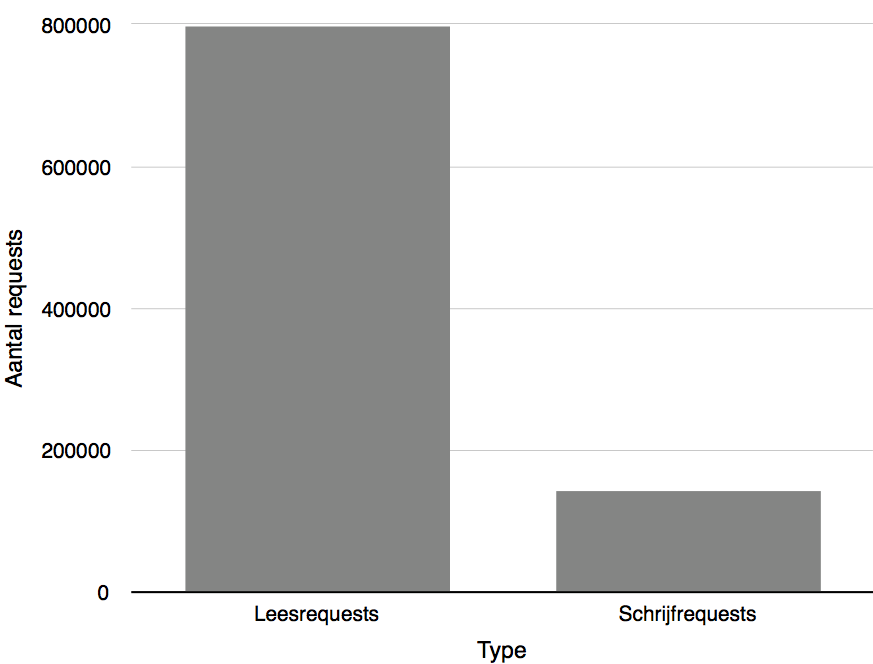
\includegraphics[width=0.75\textwidth]{img/lees-en-schrijfkant}
\end{figure}

Door de zwaardere druk langst de leeskant, kan er moeilijk geoptimaliseerd worden voor alle cases waar zowel de lees- als schrijfkant voordeel uit haalt. De splitsing is daarom een voordeel om langs beide kanten te kunnen optimaliseren.

Wanneer de lees- en schrijfkant niet gescheiden zouden worden, dan maken ze gebruik van de dezelfde databank. Wanneer er gelezen wordt en door een andere partij geschreven wordt, kan dit elkaar hinderen omdat beide kanten dezelfde resources gebruiken.

CQRS speelt en grote rol bij EventSourcing, vandaar dit korte hoofdstuk.
